\documentclass{article}
\usepackage[margin=.9in]{geometry}
\usepackage[dvipsnames]{xcolor}
\usepackage{amsmath}
\usepackage{amssymb}
\usepackage{amsthm}
\usepackage{tikz}
\usepackage{mathrsfs}
\usepackage{float}
\newtheorem*{claim}{Claim}
\newtheorem*{poof}{Proof}
\title{HW 8}
\author{Christopher Hunt}
\date{}
\usepackage{graphicx} 
\usepackage{fancyhdr}

\begin{document}
\pagestyle{fancy}
\fancyhf{}
\rfoot{MTH 231}
\lfoot{Christopher Hunt}
\lhead{HW 8}
\rhead{\thepage}
\maketitle

\section*{26. Show that the graph doesn't have a Hamilton circuit.}
\begin{center}
    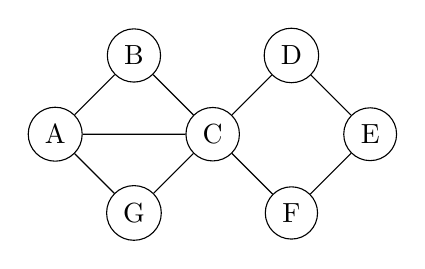
\begin{tikzpicture}
        % Draw vertices
        
        \node[circle, draw] (B) at (1, 0) {B};
        \node[circle, draw] (D) at (3, 0) {D};
        \node[circle, draw] (F) at (3, -2) {F};
        \node[circle, draw] (A) at (0, -1) {A};
        \node[circle, draw] (C) at (2, -1) {C};
        \node[circle, draw] (G) at (1, -2) {G};
        \node[circle, draw] (E) at (4, -1) {E};
      
        % Draw edges
        \draw (A) -- (B) -- (C);
        \draw (A) -- (C) -- (D) -- (E);
        \draw (A) -- (G) -- (C);
        \draw (C) -- (F) -- (E);
      \end{tikzpicture}
\end{center}

A Hamiltonian Circuit is a path in a graph that visits every vertex exactly once and ends at the starting vertex, the starting vertex can only be visited a second time to end the circuit. For the graph in question there are two different sides of the graph seperated by a common vertex C, this gives us three sets of vertices to consider. Set one consits of the set of vertices $\{A,B,G\}$, set two consists of $\{D,E,F\}$ and set three is the set $\{C\}$. This gives us three main cases to concider.

Case 1: If we begin our circuit on any vertex from set one we see that any attempt to visit the vertices in set two would require us to visit vertex C once when entering the right side of the graph and then visit vertex C a second time when attempting to return to the starting vertex in set one. This is not allowed by the definition of a Hamiltonian Circuit.

Case 2: If we begin our circuit on any vertex from set two we encounter the same problem as case 1. To visit vertices in set one we must visit vertex C once to enter the set and then visit vertex C a second time when attempting to complete the circuit. This is not allowed by the definition of a Hamiltonia Circuit.

Case 3: If we begin our circuit from set three, which is just vertex C, we see that we can either move to a vertex in set one or a vertex in set two. Once we've made this decision we fall victim to the same problem as cases 1 and 2. Any attempt to reach vertices in the set that we did not enter first requires us to move through vertex C which is not allowed by the definition of a Hamiltonian Circuit.

The vertex C acts as a choke point between two different sections of the total graph, any attempt to make a Hamiltonian Circuit would require us to visit vertex C more than the minimum required to make a Hamiltonian Circuit. Therefore the graph in question does not have a Hamiltonian Circuit.

\newpage

\section*{SQ-15b. Prove (or explain carefully why it's true) that any two spanning trees for a graph have the same number of edges.}

\hspace*{\parindent}To begin recall the definition of a tree and a spanning tree of a graph. A tree is a graph that is connected and acyclic, any two vertices in a tree are connected by exactly one path. A spanning tree of a graph is a subgraph of some graph G that is a tree and connects all the vertices in G.

Suppose we have some arbitrary connected graph $G$ which contains $n$ vertices. Let us attempt to make a subgraph of $G$ which is an arbitrary spanning tree $T$. Begin by picking an arbitrary vertex, our tree now contains 1 vertex and no edges. After this first step, every additional vertex added to the tree must be connected to the existing tree $T$ by an edge whose addition does not create a cycle. That means that the second vertex added will also bring with it an edge, the count of vertices is now 2 and the count of edges is now 1. Continue adding vertices and edges to the spanning tree, making sure no cycles are made until all vertices have been used. The total number of vertices and edges with be vertices = $n$ and edges = $n-1$.

Now, let's consider constructing another, different spanning tree $T'$ of the same graph $G$. Even though we may start from a different vertex and the order of vertex addition may differ, the core procedure is identical: start with one vertex and zero edges, and each additional vertex must be connected to the existing tree by exactly one edge, without forming a cycle. This process concludes when all vertices from $G$ have been incorporated into $T'$. Like $T$, this new spanning tree $T'$ will also have $n$ vertices and $n-1$ edges.

We can therefore conclude that any two spanning trees of a connected graph $G$ will contain the same number of edges. This is because the number of edges in a spanning tree is determined by the number of vertices in the graph and the need to maintain an acyclic, connected structure, irrespective of the specific vertices or edges chosen to form the tree.
\end{document}